{\color{gray}\hrule}
\begin{center}
\section{Spatial Hierarchical Clustering applied to DGGS: Algorithms and Complexity}
\textbf{Here we will go into detail on our algorithm design and approach for optimization of STAC queries when generating our dataset.}
\bigskip
\end{center}
{\color{gray}\hrule}

% \begin{multicols}{2}

\subsection{Data Ingestion and Pre-processing}
\label{subsec:data_ingestion}

\paragraph{Dataset Acquisition and Management} 
We download PV installation datasets from various academic repositories including Zenodo, figshare, GitHub, and ScienceBase. 
The datasets listed in the table below are publicly available and can be used for training and testing of computer vision models for PV array segmentation and detection. 
They were selected based on their availability, size, area coverage, and relevance to the problem of PV array segmentation and detection.
The data records are available in multiple vector file formats (GeoJSON, GeoPackage, Shapefile), which we standardize using our data pipeline. a
We utilize the \texttt{datahugger} library to fetch datasets from Zenodo and figshare, \texttt{sciencebasepy} for accessing the USGS ScienceBase Catalog, 
and custom functions for GitHub-hosted datasets. Dataset metadata is stored in a structured JSON configuration file to track sources, DOIs, and formats. 
For implementation details of this subsection, we refer the reader to the \href{https://github.com/avega17/CCOM_MS_Spring_2025_EO_PV_research/blob/main/fetch-pv-datasets-ESDA.ipynb}{fetch-pv-datasets-ESDA.ipynb} notebook.

\paragraph{Standardization to GeoParquet}
We convert all vector dataset files to GeoParquet format using \texttt{geopandas}. GeoParquet extends the Apache Parquet columnar storage format with geospatial capabilities, providing significant advantages:
\begin{itemize}
    \item \textit{Efficient storage} with built-in compression, reducing file sizes compared to GeoJSON and other spatial vector formats
    \item \textit{Columnar storage format} optimized for analytical queries and filtering operations
    \item \textit{Spatial indexing and predicate pushdown} capabilities for efficient geospatial operations over supported geometry types
    \item \textit{Wide ecosystem compatibility} with modern geospatial and cloud-optimized tools and workflows
\end{itemize}

This provides a space complexity reduction. For example, the cumulative size of the 5 datasets(cite) we worked with this semester was 690.5 MB in GeoJSON and GeoPackage formats, 
while after consolidation and conversion to GeoParquet the size was reduced to 107.3MB. This is largely due to the inherent compression capabilities of the Parquet format, from removing unused columns, 
and filtering out invalid geometries. 

\paragraph{Consolidation and Deduplication}
After standardizing individual datasets, we:
\begin{enumerate}
    \item Consolidate all datasets into a single DuckDB database with spatial extensions enabled
    \item Create a unified schema with standardized columns (geometry, area, source dataset, etc.)
    \item Perform spatial deduplication to remove overlapping polygons using spatial indices
    \item For CV models, filter to only retain valid polygon geometries (POLYGON, MULTI-POLYGON) for segmentation training
\end{enumerate}

The running time for the deduplication process is reduced by using spatial indices as for each record we only need to compare nearby geometries as established by the spatial index.


\paragraph{Geospatial Enrichment}
We enrich the consolidated PV dataset with administrative boundary information from the Overture Maps project:
\begin{enumerate}
    \item Spatial join with Overture divisions (countries, regions, counties)
    \item Administrative division matching (ISO country codes and region names, and division\_ids for future querying) for each PV installation
    \item Aggregation statistics at country and region levels
    \item Choropleth visualizations of PV distribution by country and region
    \item Leafmap interactive scatterplot map for visualizing PV installations coordinates in Jupyter notebooks
    \item Adding geographic context allows us to train by country or even regional models adapted to local conditions
    \item Enables efficient querying of PV installations by administrative divisions
\end{enumerate}

\paragraph{H3 Indexing and Spatial Aggregation}
To efficiently organize and query the global PV dataset, we utilize H3, the hierarchical hexagonal DGGS discussed above.
H3 provides a hierarchical structure of hexagonal grid cells, allowing for efficient spatial indexing and querying. There are \texttt{duckdb} and \texttt{python} bindings available for H3,
which we use to index the PV dataset and perform spatial operations.
\begin{enumerate}
    \item Each PV installation is assigned an H3 index at optimal resolution based on its size
    \item Common H3 resolution (level 5, $\sim$250km$^2$ hexagons) added for regional aggregation
    \item Efficient spatial clustering and adaptive subdivisions using H3 hierarchy
    \item Spatial joins with geospatial data layers (Overture Maps) using H3 indices as common keys
\end{enumerate}

\subsection{Graph Construction from H3 Grid Cells for MST [Future Work]}

A Mutual Reachibility Graph (MRG) is an undirected, weighted graph where each node represents a point in the dataset and edges represent the mutual reachability distance between points.
The foundation for our hierarchical spatial clustering is a graph $G=(V, E_w)$, where the set of vertices $V$ represents H3 grid cells containing PV installations, and $E_w$ is the set of weighted edges quantifying the proximity between these cells.

\paragraph{Node Definition}
Instead of the set of raw input data points, the geometric centroids of each unique H3 cell that contains one or more PV PoIs at a chosen analysis resolution (e.g., $res_A$) becomes a node $v \in V$. Let $N = |V|$ be the total number of such H3 cells.

\paragraph{Edge Weight Definition}
The primary metric for defining the weight (or "distance") between any two H3 cell nodes, say $c_a$ and $c_b$, is the H3 grid distance: $w(c_a, c_b) = \texttt{h3.grid\_distance}(c_a, c_b)$. 
This function returns the shortest number of steps (hops) on the H3 grid required to move from $c_a$ to $c_b$.
\begin{itemize}
    \item This topological (i.e. not geometric) distance inherently captures spatial adjacency and connectivity within the H3 grid structure. 
    The \texttt{h3.grid\_distance} function itself is efficient and can be considered $O(1)$ constant time for a single pair\cite{H3_Algorithm1}, typically operating in constant time or time proportional to the distance, as it relies on arithmetic and geometric operations on cell IDs.
    \item Using \texttt{h3.grid\_distance} directly as the edge weight prioritizes connecting H3 cells that are close in terms of grid topology for the MST.
\end{itemize}
% While this is the primary metric, future work could explore hybrid weighting schemes that incorporate feature similarity between H3 cells (e.g., similarity in PV density, installation dates, or STAC-derived land cover characteristics) in addition to the grid distance.

\paragraph{Graph Sparsification for Scalability}
A naive approach to constructing a complete graph with edges between all $N$ H3 cells would require computing $O(N^2)$ edge weights, making MST computation intractable for large $N$. Therefore, graph sparsification is essential:
\begin{enumerate}
    \item \textbf{$k$-Ring Neighbors:} For each H3 cell $c_i$, consider only edges to its immediate H3 neighbors within a small $k$-ring (e.g., using \texttt{h3.k\_ring(}$c_i$\texttt{, k\_val)} where $1 \geq k' \leq 3$). 
    This bounds the number of candidate edges to $O(N \cdot 7^{k'})$ where N is the number of H3 cells with PV installations and further bounded by only considering grid cells with PV installations.
    \item \textbf{Maximum H3 Distance Threshold:} Alternatively, consider edges only between H3 cells $c_a, c_b$ if $\texttt{h3.grid\_distance}(c_a, c_b) \leq D_{\max}$, where $D_{\max}$ is a predefined maximum H3 distance. 
    The number of edges here would depend on the spatial distribution of PV-containing H3 cells and $D_{\max}$.
\end{enumerate}
These sparsification strategies significantly reduce the number of edges ($E_{sparse}$) in the graph, typically to $O(N \cdot \text{avg\_degree})$, making subsequent MST algorithms (like Kruskal's or Prim's, which scale with the number of edges) computationally feasible. 
The choice of sparsification parameters ($k'$ or $D_{\max}$) involves a trade-off between computational cost and the fidelity of the resulting MST compared to one built on a complete graph.
The resulting sparse, weighted graph of H3 cells is the direct input to the MST construction algorithms. 

\subsection{MST Construction: Running Time and Parallel Optimizations [Future Work]}
% * Algorithm: Parallel GeoFilterKruskal (GFK) with MemoGFK optimization (Wang et al., 2021).
% * Justification: Scalability for large numbers of H3 cells, memory efficiency.
% * *(If HDBSCAN*-like density focus is explored: discuss core distance definition for H3 cells and Wang et al.'s specialized well-separation).*
\label{subsec:mst_construction}

Once the sparse graph of H3 cells $G=(V, E_{sparse})$ is constructed, the next crucial step is the construction of a MST. 
The MST will form the backbone for the subsequent hierarchical clustering and dendrogram generation as described in \cite{Wang_Yu_Gu_Shun_2021}. 
Therefore we need efficient algorithms for MST construction, especially given the potentially large number of H3 cells ($N$) involved in a global or regional analysis.

\paragraph{Classic MST Algorithms and Complexity}
Several classic algorithms are foundational for MST construction on a graph with $N$ vertices and $E_{sparse}$ edges:
\begin{itemize}
    \item \textbf{Kruskal's Algorithm:} Sorts all $E_{sparse}$ edges by weight and adds them if they connect two previously unconnected components. Complexity: $O(E_{sparse} \log E_{sparse})$ or $O(E_{sparse} \log N)$ using a Union-Find data structure.
    \item \textbf{Prim's Algorithm:} Grows the MST from a start vertex, iteratively adding the cheapest edge to an unvisited vertex. Complexity: $O(E_{sparse} \log N)$ with a binary heap, or $O(E_{sparse} + N \log N)$ with a Fibonacci heap.
    \item \textbf{Boruvka's Algorithm:} Iteratively adds the minimum weight edge incident to each component. Complexity: $O(E_{sparse} \log N)$, and is inherently parallelizable.
\end{itemize}
Given our graph sparsification, where $E_{sparse}$ is typically $O(N)$ (e.g., when using $k$-ring neighbors with small $k'$), these algorithms become significantly more tractable. For example, Kruskal's algorithm would have a complexity of roughly $O(N \log N)$.

\paragraph{Parallel Optimizations for EMST and Adaptations for H3 Graphs [Future Work]}
For Euclidean Minimum Spanning Trees (EMST) on point data, where the graph is implicitly dense, Wang et al. (2021) proposed parallel algorithms using Well-Separated Pair Decompositions (WSPDs) to reduce effective pairs to $O(N)$, and a parallel GeoFilterKruskal (GFK)\cite{Wang_Fast_Parallel_EMST_HDBSCAN_2021}. 
Their parallel EMST algorithm achieves $O(N^2)$ work in constant dimensions but, importantly, has a polylogarithmic depth, $O(\log^2 N)$, (i.e., the longest series of sequential operations in the parallel algorithm) enabling substantial parallel speedups. 

For our H3 graph, which is already sparse due to the strategies in Section \ref{subsec:graph_construction_h3}:
\begin{enumerate}
    \item Parallel versions of Kruskal's (like the author's Parallel GFK) or Boruvka's algorithm are directly applicable and offer good performance.
    \item The principle of Wang et al.'s GFK/MemoGFK (processing edges in batches based on weight ranges) can still be beneficial for managing memory and improving cache efficiency if $E_{sparse}$ remains very large (e.g., for global-scale analysis with a high average degree after sparsification).
\end{enumerate}
As the authors showed in their runtime decomposition figure, the MST Construction step has by far the shortest running time compared to their WSPD and Dendogram algorithms.
The effort in constructing the MST efficiently is well-justified as the relatively fast computation of MSTs, especially with parallel and memory optimizations on sparse graphs, makes this approach viable for large-scale, planetary datasets of H3 cells.

\subsection{Generating a Hierarchy of Clusters: Dendrogram Construction and H3 Multi-resolution}
\label{subsec:dendrogram_construction}

Following construction of the MST from H3 cells, the next step is to derive a hierarchy of clusters. 
This is achieved by generating a dendrogram, which visually and structurally represents the nested groupings of H3 cells based on their proximity or similarity as captured by the MST. 
The dendrogram is fundamental to hierarchical clustering, allowing for the exploration of cluster structures at various levels of granularity and informing our selection of STAC raster assets.

\paragraph{Dendrograms from MSTs}
A single-linkage dendrogram can be directly constructed from an MST. Conceptually, if MST edges are sorted by weight (e.g., \texttt{h3.grid\_distance}), the dendrogram represents 
the sequence of merges (in an agglomerative sense) or splits (in a divisive sense) of H3 cells. Each internal node in the dendrogram corresponds to an edge in the MST, and 
its height in the dendrogram is typically proportional to the weight of that edge. Cutting the dendrogram at a certain height yields a flat partitioning of the H3 cells into $k$ clusters.

\paragraph{Efficient Dendrogram Construction}
Traditionally, dendrograms are built sequentially, often using a Union-Find data structure, which for large $N$ (number of H3 cells) can be a bottleneck ($O(N \log N)$ but serial). 
For the scope of this project, we briefly highlight the development of parallel algorithms for Single-Linkage Dendrogram (SLD) computation that offer improved theoretical guarantees and practical speedups. 
For instance, algorithms by Dhulipala et al. (2024) achieve $O(N \log h)$ work (where $h$ is dendrogram height) with practical CPU implementations like RC-Tree Tracing (RCTT) \cite{dhulipala_Optimal_Parallel_Dendrogram_2024}. 
Furthermore, PANDORA (Sao et al., 2024) provides a work-optimal ($O(N \log N)$) GPU-accelerated approach robust to skewed dendrograms \cite{sao_PANDORA_GPU_Dendrogram_2024}. 
The use of such efficient methods is crucial for handling the scale of H3 cell datasets derived from global PV PoIs, ensuring the dendrogram generation step does not act as a bottleneck for the overall workflow 
as shown in Wang et al.'s runtime decomposition figure \cite{Wang_Fast_Parallel_EMST_HDBSCAN_2021} below.

\subsection{Optimized STAC Querying [Future Work]}

\paragraph{Integrating H3 Hierarchy for Optimized STAC Asset Selection and Coverage}
The primary focus is on leveraging the resulting hierarchy in conjunction with H3's hierarchical capabilities to efficiently generate the MST-based geometries used for querying STAC assets.
While the MST-derived dendrogram provides a \textit{data-driven hierarchy} of PV-containing H3 cells, Uber H3's native hierarchical functions are instrumental in \textbf{relating these clusters to STAC raster asset extents and administrative boundaries} (e.g., countries). 
This integration is key to optimizing the selection of STAC assets to maximize PV coverage while minimizing data redundancy for initial querying, and then enabling selective accumulation of imagery for analysis.

\begin{enumerate}
    \item \textbf{Representing STAC Raster Footprints with H3 and joining with PV H3 cells:}
        For each candidate STAC raster Item, its geographic footprint (a bounding box polygon) is converted into a set of H3 cells at a chosen base analysis resolution (e.g., $res_A$) using the \texttt{h3.polygon\_to\_cells(h3shape, res)} function. 
        This creates a \textit{discrete, gridded representation of each raster's coverage}.

    \item \textbf{Contextualizing Raster H3 Cells with AOI Geometries:}
        The H3 cells derived from STAC raster polyfills of H3 cells are then spatially intersected with the geometry of an Area-of-Interest (AOI) (from Overture Maps \textit{division\_area} theme) which we convert to H3 Cells using the same function. 
        This step identifies, for each AOI, the subset of H3 cells from each overlapping raster that falls within its boundaries. We specifically only track raster-derived H3 cells that also correspond to H3 cells containing our PV PoIs. 
        In this way we can capture only the "cells of Interest" (COIs) for each STAC raster item and AOI.
        
        \begin{figure}[ht]
            \centering
            \begin{subfigure}{\textwidth}
                \centering
                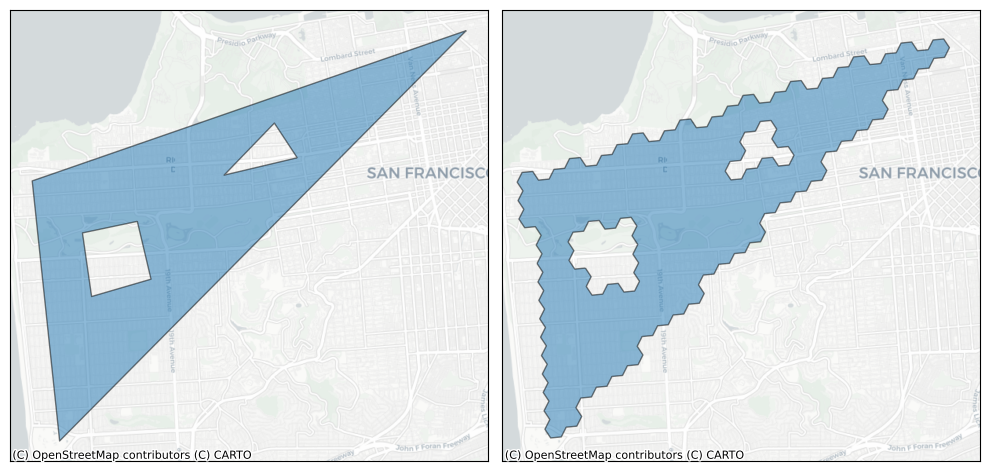
\includegraphics[width=0.6\textwidth]{report/assets/figures/h3_polygonToCells_example_res9.png}
                \caption{Polyfill of H3 cells at resolution 9 of an example Polygon}
            \end{subfigure}
            
            \begin{subfigure}{\textwidth}
                \centering
                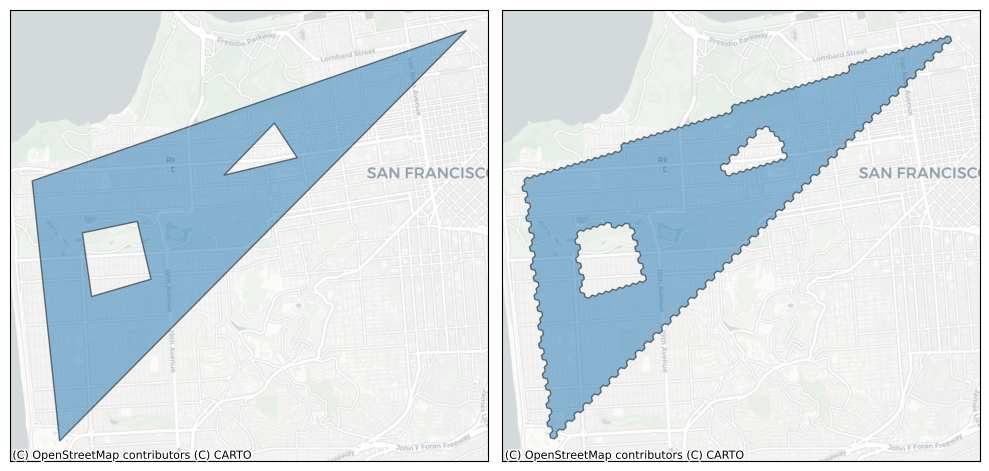
\includegraphics[width=0.6\textwidth]{report/assets/figures/h3_polygonToCells_example_res10.png}
                \caption{Polyfill of H3 cells at resolution 10 of the same example Polygon with higher precision}
            \end{subfigure}
            % \caption{Representation of a STAC item footprint at different H3 resolutions using \texttt{polygon\_to\_cells()}. Higher resolutions provide more precise coverage representation at the cost of more cells.}
            \label{fig:h3_polygon_to_cells}
        \end{figure}

        Since we are simply accumulating counts and logging raster item ID's to each H3 cell, these operations lend themselves to simple SQL aggregation queries in \texttt{duckdb} using the available H3 duckdb bindings. 
        This lets us trivially vectorize and parallelize the aggregation process over vast STAC collections once the STAC catalogs \texttt{json} files are retrieved. 
        This can be further optimized by converting STAC \texttt{json} collections to geoparquet using \texttt{stac-geoparquet} which allows for efficient processing and analytics over STAC items in bulk. 

    \item \textbf{Optimizing Raster Coverage Representation using \texttt{h3.compact\_cells()}:}
        \textit{For each STAC raster asset}, its set of H3 cells (derived and filtered as described above) can be further optimized.
        The \texttt{h3.compact\_cells()} function takes this set of fine-resolution H3 cells and returns a \textit{minimal set of H3 cells}, at coarser (parent) resolutions if all children cells are present, that \textit{approximately cover the original set of cells}.
        This creates \textbf{a concise, multi-resolution representation of each raster's effective coverage of PV POIs within a given AOI}. 
        This is particularly useful as, for our usecase, STAC asset footprints (i.e. satellite image strips over a curved surface) are often irregular and may not align neatly with a single H3 resolution. 

    \item \textbf{Relating Compacted Raster Representations to H3-MST Clusters:}
        The H3-MST and its derived dendrogram define clusters of PV-containing H3 cells themselves contained within a given division geometry. 
        The core optimization problem is to select a minimal subset of STAC rasters (represented by their compacted H3 cells footprints) that collectively maximize coverage over these PV H3 cells and the broader AOI being surveyed for PV development.
        \begin{itemize}
            \item The dendrogram provides a hierarchical view of PV cluster significance and spatial scale. Broad, extensive clusters (higher in the dendrogram, formed by merging along higher-weight MST edges) 
            can guide the selection of STAC items that offer wide-area coverage, represented by larger or more numerous compacted H3 cells.
            \item Finer, more localized clusters (lower in the dendrogram) help ensure that STAC items providing more granular or specific coverage are also considered, particularly if broad coverage assets miss these details.
            \item The selection process thus becomes a guided search, where the H3-MST cluster structure informs the value (in terms of PV coverage) of including a particular STAC asset in our collection for further analysis. 
            The emphasis is on achieving comprehensive coverage by potentially multiple rasters over the same H3 cells, rather than strict minimization of overlap if these overlaps provide valuable temporal or quality variance (e.g. cloud cover, sun angle, sensor resolution). 
        \end{itemize}

    \item \textbf{Iterative Asset Selection, Coverage Maximization, and Training Data Curation:}
        An iterative approach is employed to build a collection of relevant STAC assets and curate training data from the "stack" of imagery available for each H3 cell of interest:
        \begin{enumerate}
            \item \textbf{Initial Asset Identification:} Identify STAC rasters whose compacted H3 representations cover high-priority PV clusters (or a large number of PV-containing H3 cells). For each such H3 cell, associate all STAC raster Items that cover it.
            \item \textbf{Iterative Coverage Expansion \& Accumulation:} Iteratively identify additional STAC rasters to ensure comprehensive coverage of all PV clusters and individual PV H3 cells. 
            For each H3 cell, accumulate a list of all STAC Items that provide coverage. This allows for building a "stack" of observations for each H3 cell, rather than discarding overlapping rasters.
            \item \textbf{H3 Hierarchy for Coverage Assessment:} During this process, H3 functions like \texttt{h3.h3\_to\_parent()} and \texttt{h3.cell\_to\_children()} assist in understanding the multi-scale coverage provided by the accumulated STAC assets for each PV H3 cell and cluster. 
            This can help in summarizing the available imagery at different granularities.
            \item \textbf{Curating Positive and Negative Training Samples from Accumulated Assets:}
            \begin{itemize}
                \item \textbf{Positive Samples:} For each PV-containing H3 cell, multiple STAC raster assets might provide coverage. 
                From this "stack" of observations, select the best quality image chip(s) for training. Selection criteria can be based on STAC item metadata (e.g., minimizing cloud cover, specific date ranges, optimal sun azimuth/elevation angles, desired sensor type, or spatial resolution). 
                \item \textbf{Negative Samples (Hard Negatives):} To improve the robustness of downstream Computer Vision models to false positives, spatially correlated negative samples are crucial\cite{kruitwagen_global_inventory_pv_units_2021, robinson_ms_planet_global_renewables_watch_2025, yang_GloSoFarID_2024}\cite{feng_10m_S2_China_2024}. 
                These are generated by:
                    \begin{enumerate}
                        \item \textbf{Materializing MST Edge Paths:} For edges in the H3-MST connecting two PV-containing H3 cells (say \texttt{cell\_A} and \texttt{cell\_B}), materialize the path of H3 cells between them using \texttt{h3.grid\_path\_cells(cell\_A, cell\_B)}. These "edge path cells" represent the immediate spatial context and are less likely to contain primary PV installations themselves. 
                        "Thin" edges in the MST (those connecting H3 cells at the finest analysis resolution, implying close \texttt{h3.grid\_distance}) are particularly good candidates for sourcing negative samples as they are likely to be visually similar to the PV cells they connect but not contain PV installations.
                        \item \textbf{Selecting Imagery for Negative Samples:} Identify which of the accumulated STAC raster assets cover these materialized edge path H3 cells. From the "stack" of observations for these negative sample H3 cells, sample suitable image chips. 
                        \item \textbf{Optional Refinement:} Further refine these negative samples by applying simple scene classification model or CV template matching against nearby confirmed PV arrays to ensure they represent "hard negatives" 
                        (areas that might share some visual characteristics with PV sites but are not). 
                    \end{enumerate}
            \end{itemize}
        \end{enumerate}
        The aim of this iterative process is to \textbf{efficiently gather a comprehensive collection of STAC raster assets covering all PV areas of interest} and, from this collection, to curate a high-quality, diverse set of image chips for both 
        positive (PV-containing H3 cells) and negative (contextual/edge H3 cells) training samples. This approach embraces the idea of leveraging multiple observations where available, akin to building a localized ``data cube'' (cite) for each H3 cell of interest. 
\end{enumerate}
This synergistic use of the MST-derived dendrogram (for identifying PV clusters) and H3's hierarchical functions (for representing STAC asset coverage, guiding asset accumulation, and curating training data) 
forms a powerful strategy for targeted and efficient analysis of large-scale EO data archives.

% \end{multicols}

\clearpage

